\documentclass[border=4pt]{standalone}
% Shared typography and colours for the standalone figures.
\usepackage{unicode-math}
\setmainfont{TeX Gyre Termes}
\setmathfont{TeX Gyre Termes Math}
\usepackage{tikz}
\usetikzlibrary{arrows.meta,positioning,calc,decorations.pathreplacing}
\usepackage{pgfplots}
\pgfplotsset{compat=1.18}

% One colour per element or subsystem. Record the mapping in
% the working repository conventions and use it identically in every figure.
\definecolor{elemA}{HTML}{1F5FA8}
\definecolor{elemB}{HTML}{B8461B}
\definecolor{elemC}{HTML}{2E7D32}
\definecolor{elemD}{HTML}{6A4C93}
\definecolor{frameline}{HTML}{555555}

\begin{document}
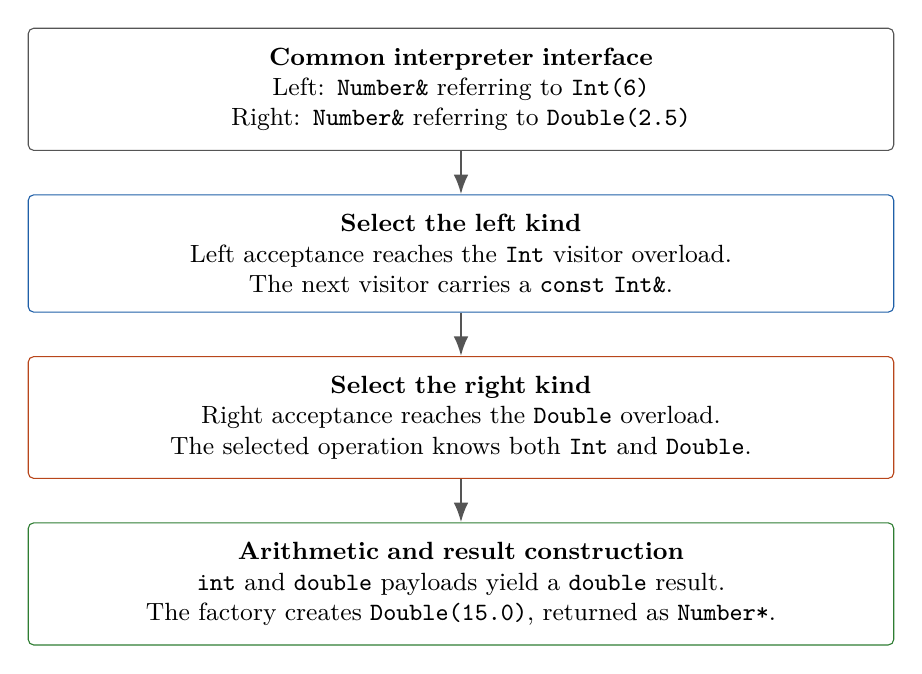
\begin{tikzpicture}[
  box/.style={draw,rounded corners=2pt,align=center,text width=10.5cm,
              minimum height=1.0cm,inner sep=7pt,font=\small},
  link/.style={-{Latex[length=2.5mm]},thick,draw=frameline}
]
\node[box,draw=frameline] (input)
  {\textbf{Common interpreter interface}\\
   Left: \texttt{Number\&} referring to \texttt{Int(6)}\\
   Right: \texttt{Number\&} referring to \texttt{Double(2.5)}};
\node[box,draw=elemA,below=0.55cm of input] (left)
  {\textbf{Select the left kind}\\
   Left acceptance reaches the \texttt{Int} visitor overload.\\
   The next visitor carries a \texttt{const Int\&}.};
\node[box,draw=elemB,below=0.55cm of left] (right)
  {\textbf{Select the right kind}\\
   Right acceptance reaches the \texttt{Double} overload.\\
   The selected operation knows both \texttt{Int} and \texttt{Double}.};
\node[box,draw=elemC,below=0.55cm of right] (operation)
  {\textbf{Arithmetic and result construction}\\
   \texttt{int} and \texttt{double} payloads yield a \texttt{double} result.\\
   The factory creates \texttt{Double(15.0)}, returned as \texttt{Number*}.};
\draw[link] (input)--(left);
\draw[link] (left)--(right);
\draw[link] (right)--(operation);
\end{tikzpicture}
\end{document}
